%----------------------------------------------------------------------
% Missuse parts as chapters according to DESY PR
\part[Part slide]{Machine Learning}
\makepart%


\begin{frame}
    \frametitle{Role of ML}
    \begin{itemize}[<+->]
        \setlength\itemsep{1em}
        \item Will start considering coordinate space: $\ket{\psi} \equiv \psi(x)$
        \item Define augmented basis as:
            \begin{equation}
                \varphi_k^A(x) = \varphi_k(g(x)) \cdot \sqrt{\det\left|\frac{\dd g}{\dd x}\right|}
            \end{equation}
        \item $g$ is a \textbf{Normalizing Flow}
        \item This preserves orthonormality
            \begin{proof}
                \[
                    \inner{\varphi_k^A(x)}{\varphi_k^A(x)} = 
                    \int \dd x \varphi_i(g(x))\varphi_j(g(x)) \cdot \det\left|\frac{\dd g}{\dd x}\right|=
                    \int \dd g \left|\frac{\dd x}{\dd g}\right| \varphi_i(g)\varphi_j(g) \cdot \det\left|\frac{\dd g}{\dd x}\right|= \delta_{i, j}
                \]
            \end{proof} 
    \end{itemize}
\end{frame}

\begin{frame}
    \frametitle{Normalizing Flows}
    \begin{itemize}[<+->]
        \setlength\itemsep{1em}
        \item Basic idea: A chain of diffeomorphisms
        \item Invertible and differentiable
        \begin{equation*}
            \boldmath{z} = (f_n\circ f_{n-1} \circ \dots \circ f_1 )(\boldmath{x})
        \end{equation*}
        \item Several different paradigms
        \item Need to find which ones best improve flexibility of basis states
        \item We concentrate on RNVP 
    \end{itemize}
\end{frame}

\begin{frame}
    \frametitle{RNVP}
    \begin{itemize}
        \setlength\itemsep{.6em}
        \item The Real-valued Non-Volume-Preserving Normalizing Flow
        \item Let $\mathcal{P}_k$ be a projection over half of the basis vectors and $\mathcal{Q}_k \equiv \mathbb{1} - \mathcal{P}_k$
        \item layer $g_k(x)$ is given by 
            \begin{equation}
                g_k(x) = \mathcal{P}_k[x] + \mathcal{Q}_k [f_k(x)] \quad \text{with} \quad f_k(x) =  e^{s_k(\mathcal{P}_k[x])} \odot x + t_k(\mathcal{P}_k[x])
                \label{eq:layer_RNVP}
            \end{equation}
        % \item The inverse of $g \equiv g_M\circ g_{M-1}\circ \dots \circ g_1$ is $g^{-1} = g_M^{-1} \circ g_{M-1}^{-1} \circ \dots \circ g_1^{-1}$
    \end{itemize}
    \begin{columns}
        \begin{column}[t]{0.48\textwidth}
            \begin{itemize}
                \item Each $g_k$ is invertible: 
                \[
                    g_k^{-1}(z) = \mathcal{P}_k[z] + \mathcal{Q}_k[f_k^{-1}(z)] 
                \]
                \[ 
                    \text{with} \quad f_k^{-1}(z) =  e^{-s_k(\mathcal{P}_k[z])} \odot (z - t_k(\mathcal{P}_k[z]))
                \]
                \item Can be shown rigorously
                % \item sub Recall that for a projection $\mathcal{P}$, we have $\mathcal{P}^2 = \mathcal{P}$
                % \item sub Using linearity of $\mathcal{Q}$ and noticing it commutes with diagonal matrices
            \end{itemize}
        \end{column}

        \begin{column}[t]{0.48\textwidth}
            \begin{figure}
                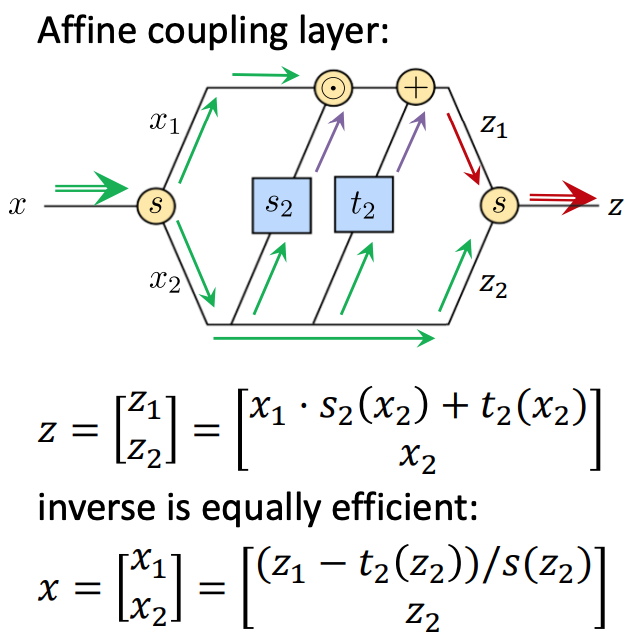
\includegraphics[width=\textwidth]{img/RNVP-basic-layer.png}
            \end{figure} 
        \end{column}
    \end{columns}

\end{frame}